\lstinputlisting[language=bash,basicstyle=\small]{python_codes/fieldstone_72/keywords}

\begin{center}
Code at \url{https://github.com/cedrict/fieldstone/tree/master/python_codes/fieldstone_72}
\end{center}

\par\noindent\rule{\textwidth}{0.4pt}

%%%%%%%%%%%%%%%%%%%%%%%%%%%%%%%%%%%%%%%%%%%%%%%%%%%%%%%%%%%%%%%%%%%%%%%%%%%%%%%%%%%%%%%%%%%%%%%%%%%%

\subsubsection*{Manufactured solution}

The analytical solution originates in Lamichhane (2015) \cite{lami15} and is 
presented in Section~\ref{ss:mms11}. 
The quadrilateral MINI element used here also originates in the same article 
and comes in two flavours with two different bubble functions $b_1$ and $b_2$
as explained in Section~\ref{ss:quadmini}.
The velocity and pressure fields are shown hereunder:

\begin{center}
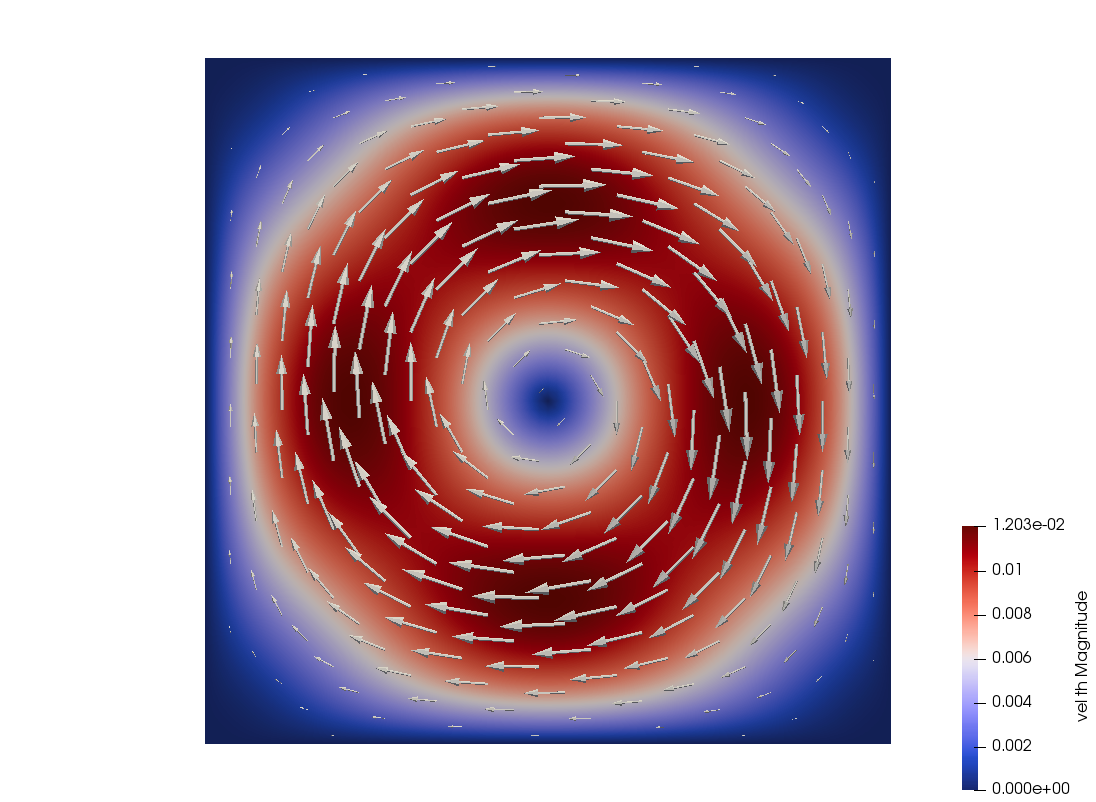
\includegraphics[width=7cm]{python_codes/fieldstone_72/results/mms/vel}
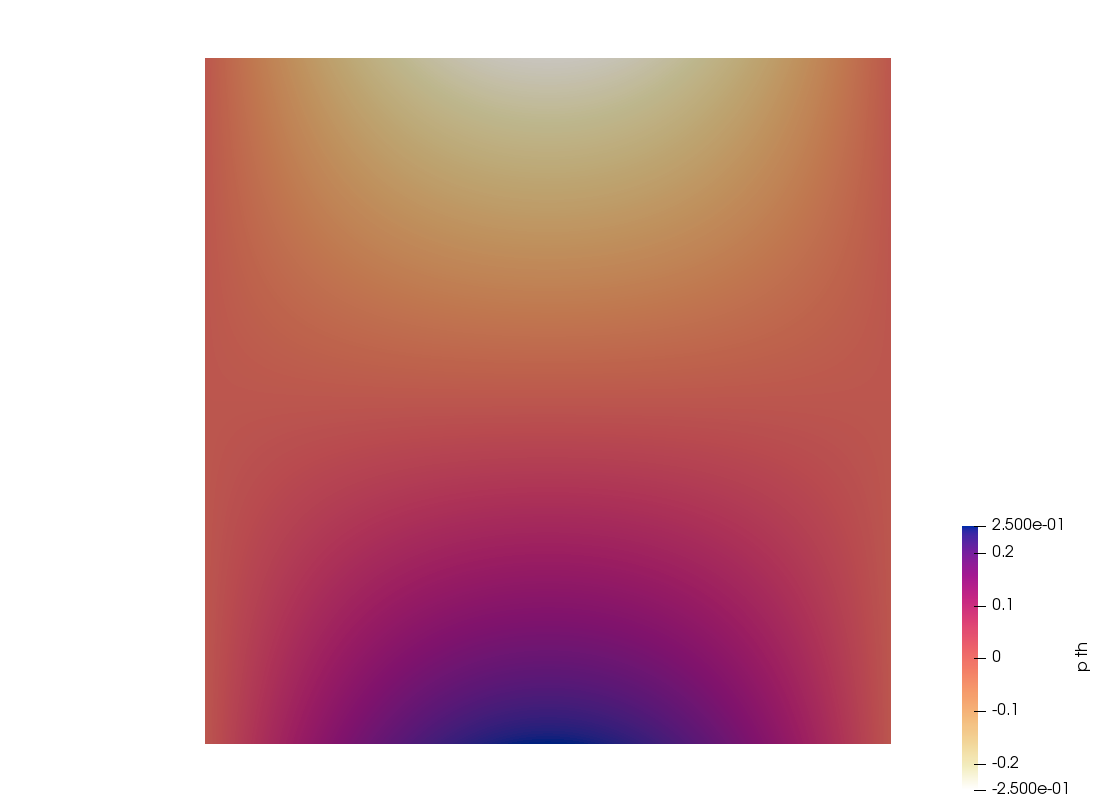
\includegraphics[width=7cm]{python_codes/fieldstone_72/results/mms/p}
\end{center}

During the debugging process I ended up 
implementing various quadratures, from $2^2$ to $6^2$ points. 
The results from the article are different than mine but I suspect that what the 
author measured could be different than what I measure. 
The trends are similar with $b_2$ performing better than $b_1$ (and 
we also observe that the quadrature scheme does not alter results at all): 

\begin{center}
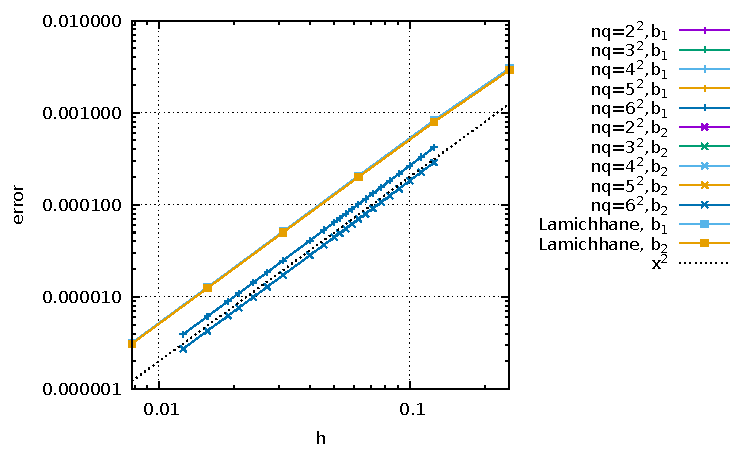
\includegraphics[width=7cm]{python_codes/fieldstone_72/results/mms/errors_v}
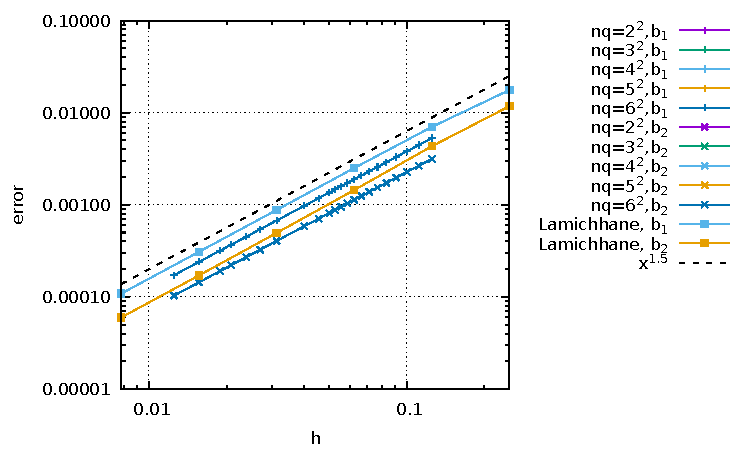
\includegraphics[width=7cm]{python_codes/fieldstone_72/results/mms/errors_p}\\
{\captionfont Left: velocity error in $L_2$ norm; Right: pressure error in $L_2$ norm.\\
Resolutions from $8\times8$ until $80\times80$.}
\end{center}

The root mean square velocity is also measured for both bubble functions.
As above we see that $b_2$ performs better than $b_1$:
\begin{center}
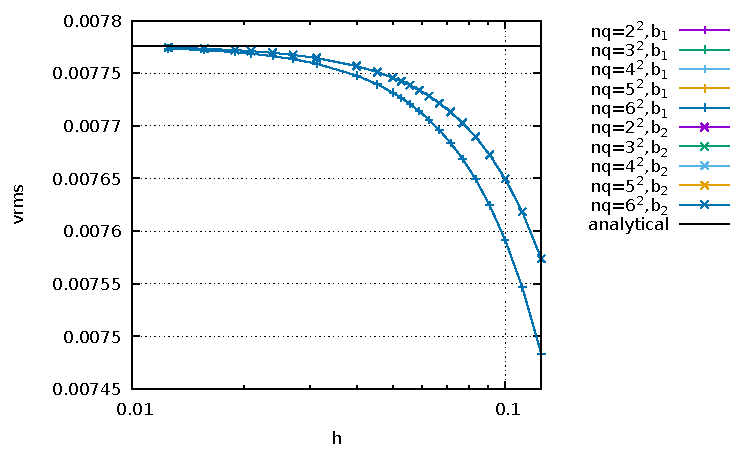
\includegraphics[width=10cm]{python_codes/fieldstone_72/results/mms/vrms}
\end{center}

%_____________________________________
\subsubsection*{Sinking block}

This is the very same experiment as in Stone 53.

%............................
\underline{Full density} 
Results indicate that the element performs adequately, especially the 
pressure field which looks smooth.  

\begin{center}
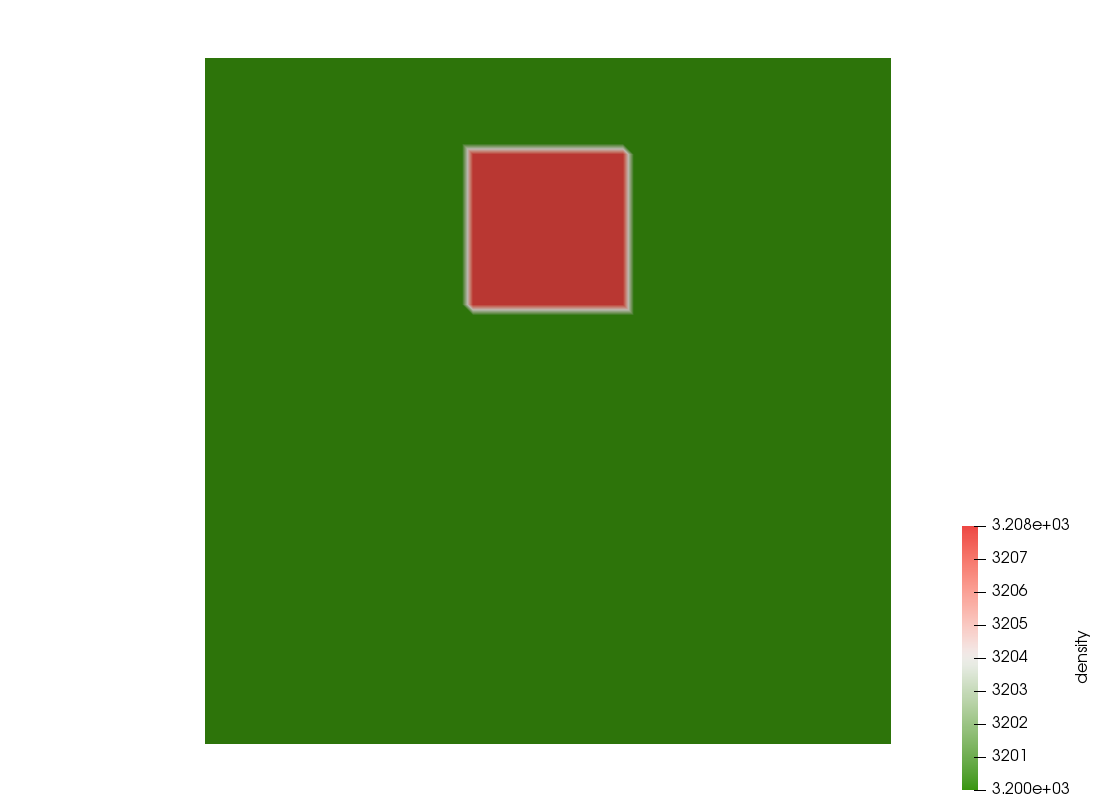
\includegraphics[width=7cm]{python_codes/fieldstone_72/results/block/full/density}
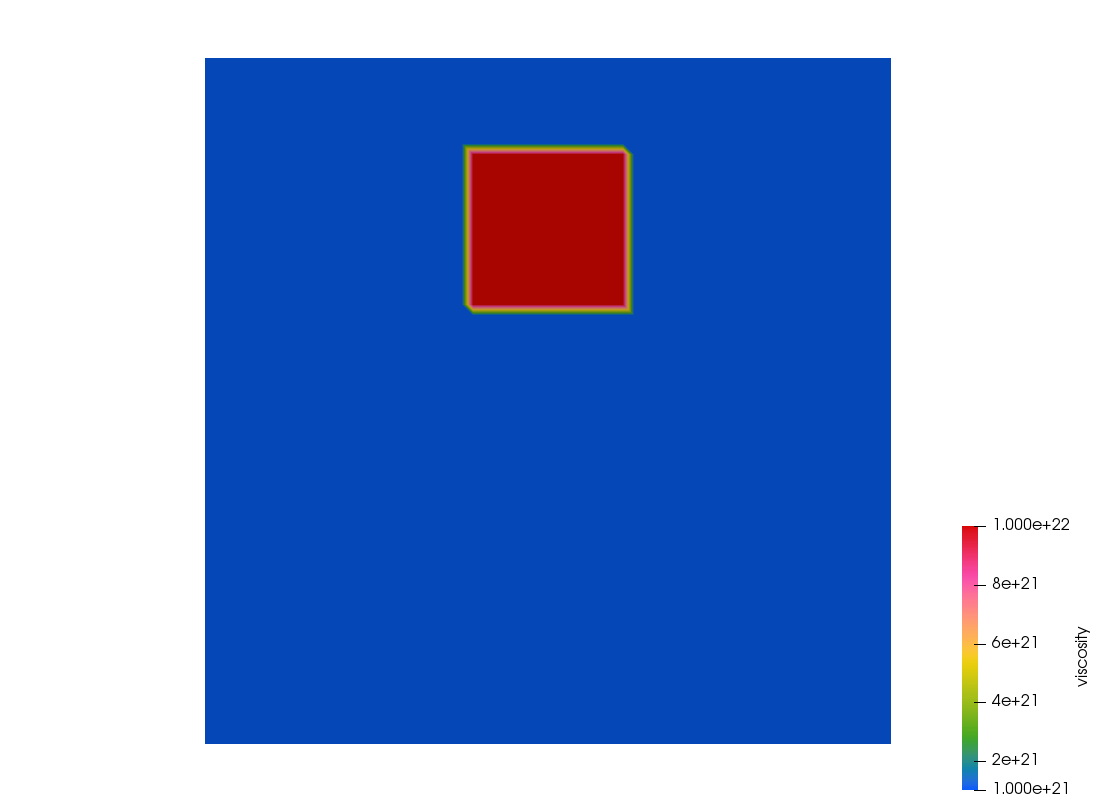
\includegraphics[width=7cm]{python_codes/fieldstone_72/results/block/full/viscosity}\\
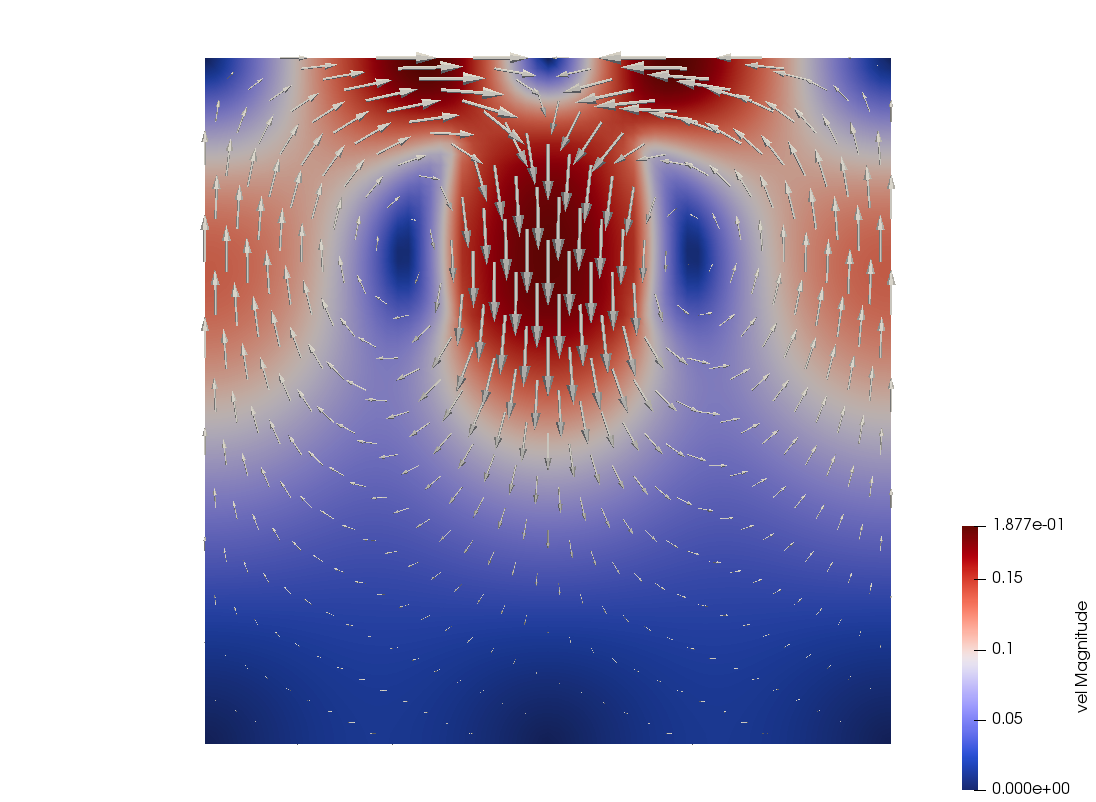
\includegraphics[width=7cm]{python_codes/fieldstone_72/results/block/full/vel}
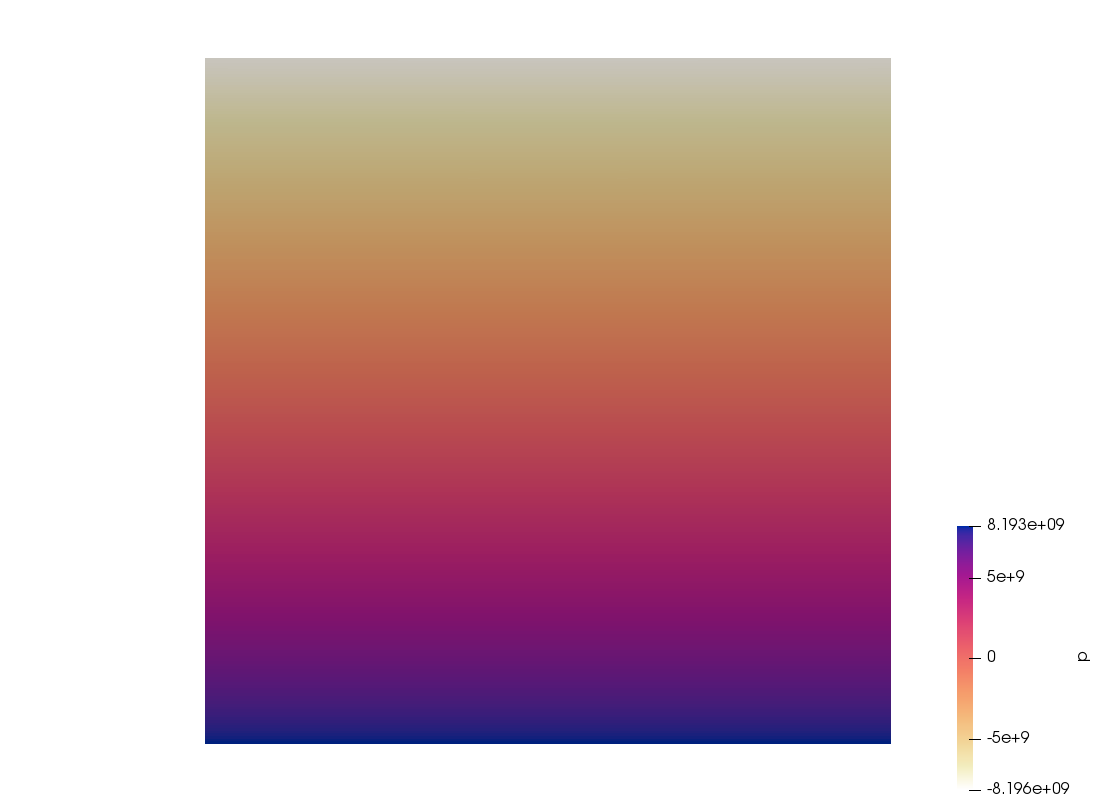
\includegraphics[width=7cm]{python_codes/fieldstone_72/results/block/full/p}\\
{\captionfont $64\times 64$. Viscosity ratio is 10, $\delta \rho=8$, bubble 1.}
\end{center}


\begin{center}
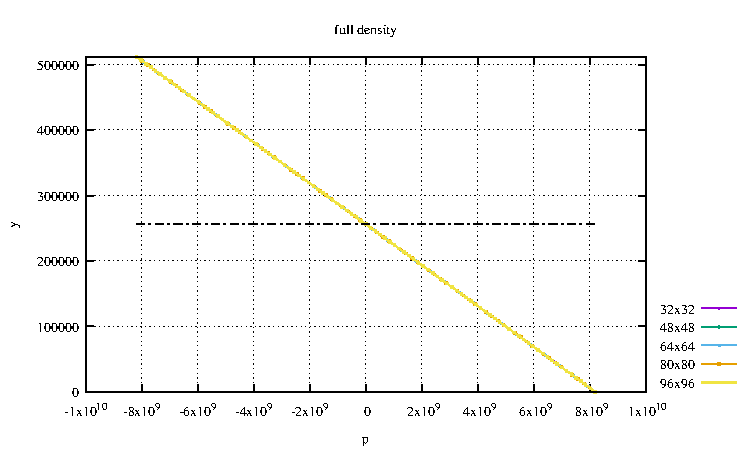
\includegraphics[width=10cm]{python_codes/fieldstone_72/results/block/full/plines}\\
{\captionfont Pressure profile measured at $x=L_x/2$ for various resolutions. Same parameters
as previous figure.}
\end{center}

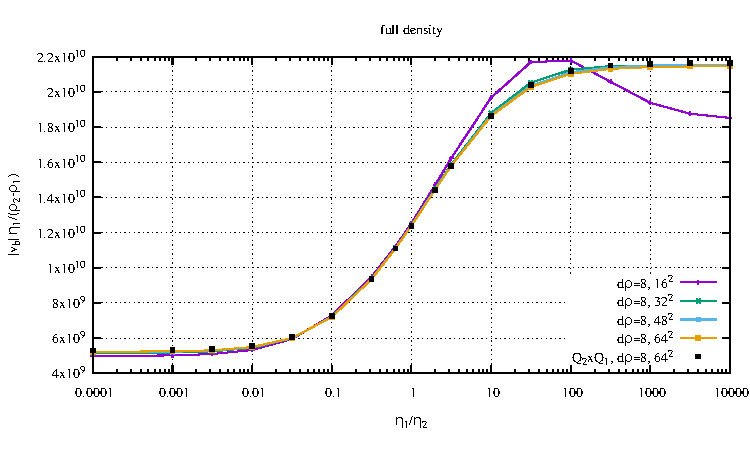
\includegraphics[width=7cm]{python_codes/fieldstone_72/results/block/full/results_v}
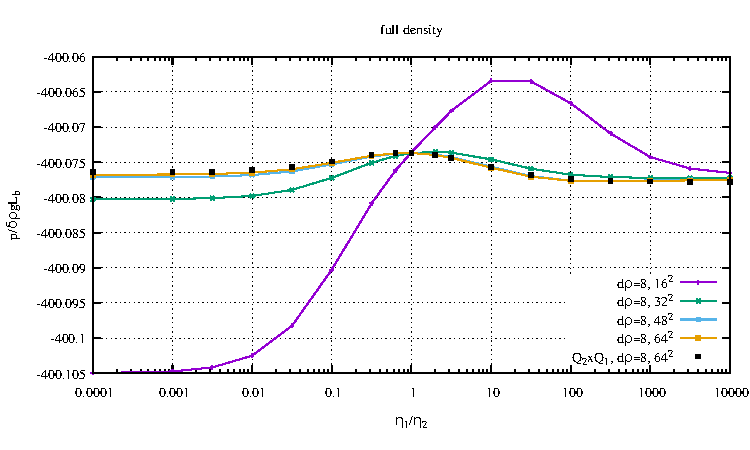
\includegraphics[width=7cm]{python_codes/fieldstone_72/results/block/full/results_p}

%............................
\underline{Reduced density} 
This is the same experiment as above but $\rho_1$ has been removed from the density
everywhere in the domain, so that the surrounding material has zero density 
and the block has a density $\delta \rho$.


\begin{center}
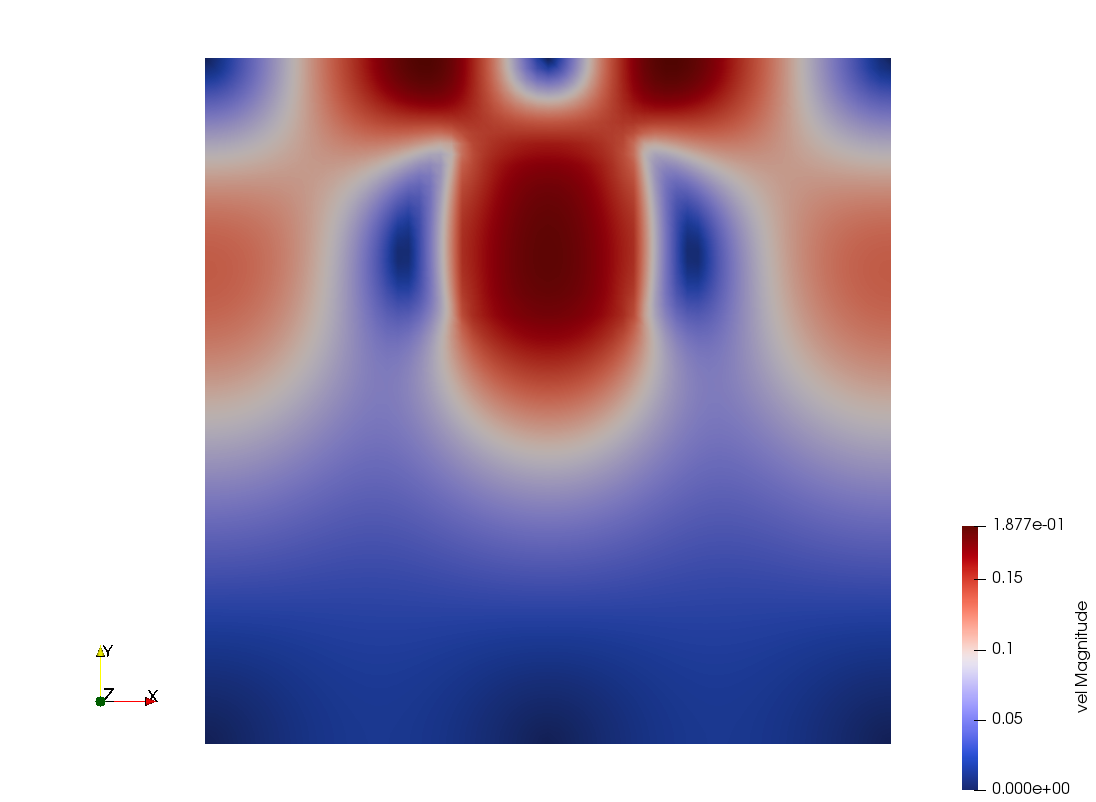
\includegraphics[width=7cm]{python_codes/fieldstone_72/results/block/reduced/vel}
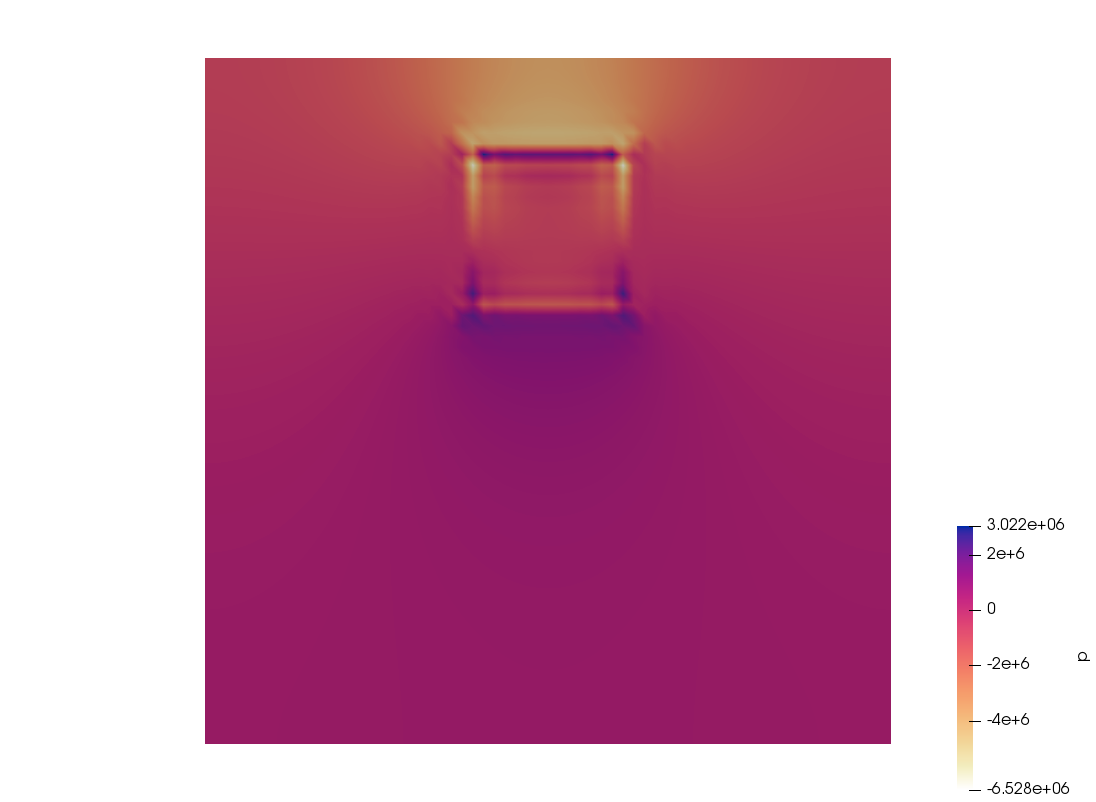
\includegraphics[width=7cm]{python_codes/fieldstone_72/results/block/reduced/p}\\
{\captionfont $64\times 64$. Viscosity ratio is 10, $\delta \rho=8$. bubble 1}
\end{center}

\begin{center}
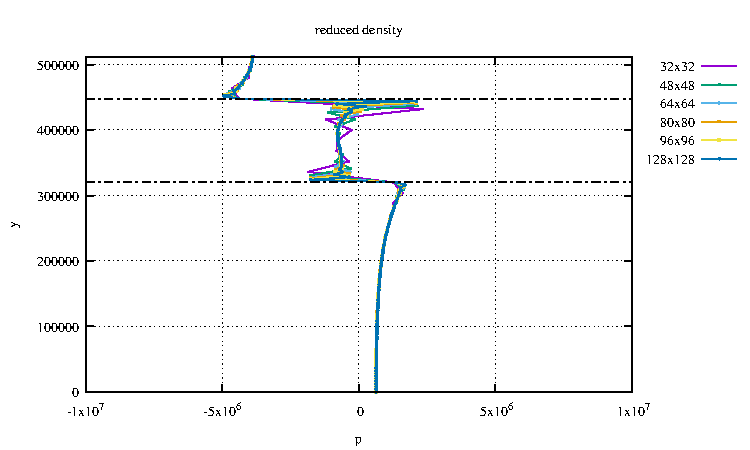
\includegraphics[width=7cm]{python_codes/fieldstone_72/results/block/reduced/plines_b1}
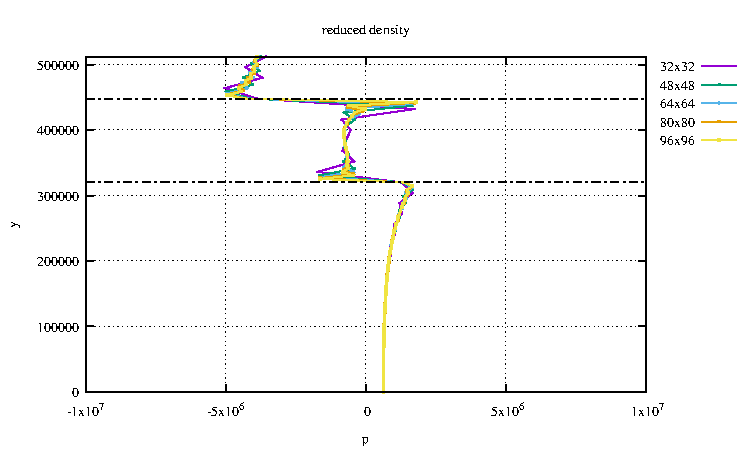
\includegraphics[width=7cm]{python_codes/fieldstone_72/results/block/reduced/plines_b2}\\
{\captionfont Pressure profile measured at $x=L_x/2$ for various resolutions and for both bubble functions.
Left is bubble 1, right is bubble 2.}
\end{center}

I hereafter plot the pressure profiles for both bubble functions at the highest resolution, i.e. $96\times 96$.
We see that differences are somewhat minimal, although bubble 2 yields a pressure above the block which 
showcases worrying oscillations:

\begin{center}
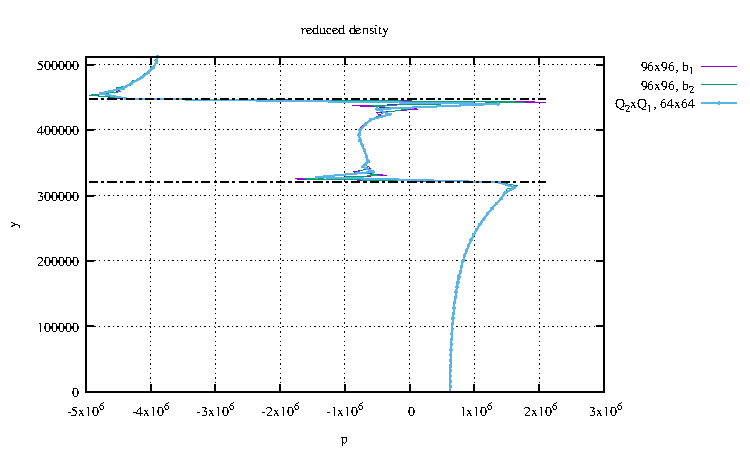
\includegraphics[width=7cm]{python_codes/fieldstone_72/results/block/reduced/plines_b12}
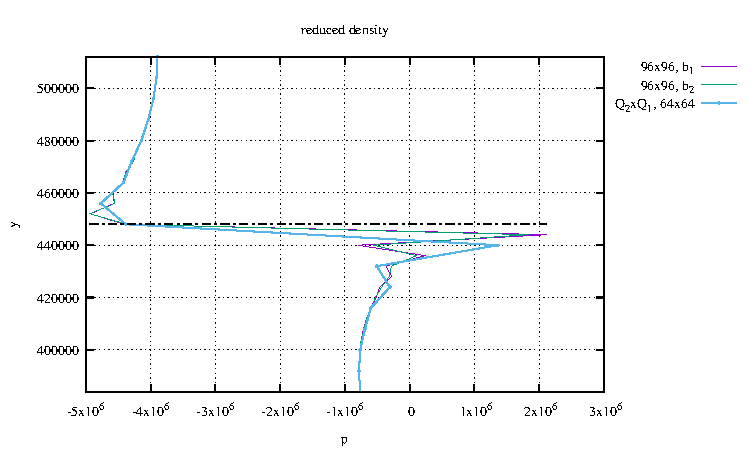
\includegraphics[width=7cm]{python_codes/fieldstone_72/results/block/reduced/plines_b12_zoom}
\end{center}



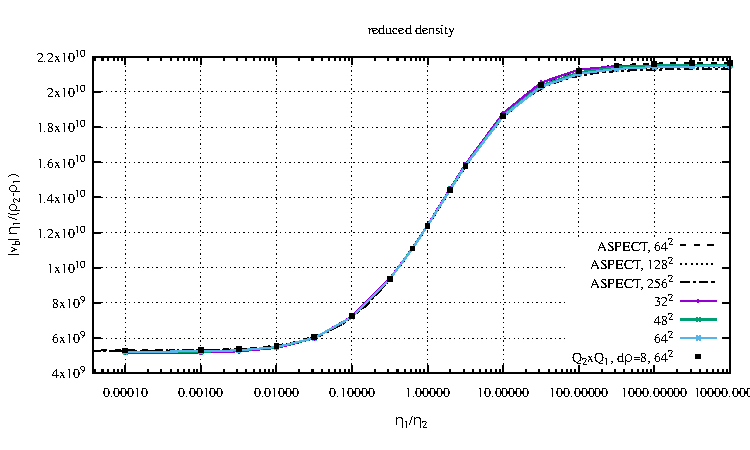
\includegraphics[width=7cm]{python_codes/fieldstone_72/results/block/reduced/results_v}
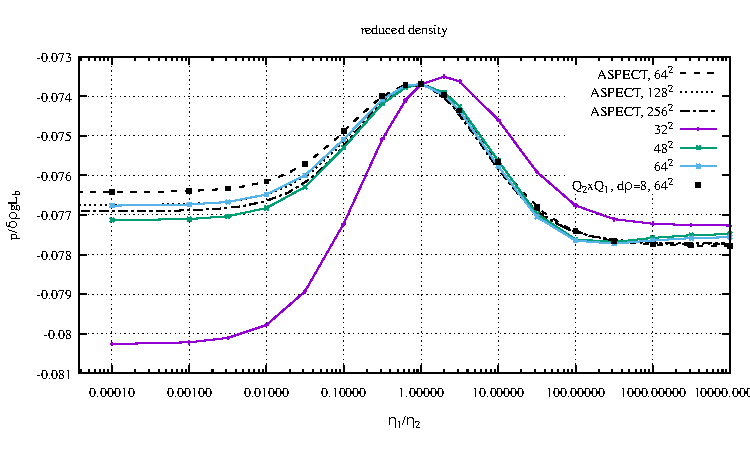
\includegraphics[width=7cm]{python_codes/fieldstone_72/results/block/reduced/results_p}



